\chapter[Introduction]{Introduction}
With the advance of technology, music - and musical instruments - have also evolved to
use it's advantages. They are a lot of use cases, the most noticeable ones being music
annotation and creation (through electronic instruments, also known as synthesizers).
All of the modern musical software and hardware use the same format to communicate,
called MIDI.

To translate music playing it is needed to know which note is being played at a
given time. This make it very easy to translate instruments that have separated
keys for each note (the most noticeable one being piano) to MIDI, but very hard
do the same for instruments like the guitar, that have a single output for multiple
notes (each string has about 15 notes). The guitar is also a harmonic instrument,
as it can play multiple notes simultaneously, which makes it's digitization even harder.

There are already a few commercial solutions for this, but not a very performant
and cheap one. Recently, a new pure software solution was released at a reasonable
price which works very well for live MIDI playing, but not enough for music annotation.
There are also a few hardware solutions available at the market, which perform well,
but are very expensive. \autoref{market-solutions} shows the most relevant solutions
in the current market.

\begin{table}[htb]
  \begin{center}
    \ABNTEXreducedfont
    \caption[Market Solutions]{Market Solutions}
    \label{market-solutions}
    \begin{tabular}{m{4 cm} | m{1 cm} | m{2 cm} | m{2 cm} | m{2 cm} }
      \hline
      Name & Price (US\$) & \pbox{2 cm}{Usage\\Complexity} & \pbox{2 cm}{Live\\Performance} & \pbox{2 cm}{Annotation\\Performance}\\
      \hline \hline
      Roland GK3 + GhostHexpander + GI20 & 700 & Hard & High & High \\
      Godin Freeway + GhostHexpander + GI20 & 800 & Hard & High & High \\
      Jam Origin - Audio to MIDI & 100 & Easy & High & Low/Medium \\
      Migic & 40 & Easy & Medium & Low \\
      \hline
    \end{tabular}
    \legend{Source: authors}
  \end{center}
\end{table}

The price for such technologies as listed in \autoref{market-solutions} may not be viable for every one,
thus the necessity of building a new product with a good performance and low price.
Our current prototype price is US\$ 77.66 (\autoref{Prototype-cost}), with estimated
production cost of US\$ 40.21 (\autoref{Production-cost}) for each of 1000 units. This can lower (about 30 dollars) if using
a cheaper amplifier circuit. The numbers listed show how this project can be viable
as a product. 

A great amount of technology needs to be built around this project as software, which
can also foment a market grow for this kind of product and therefore create space for
new ideas in the area. The area around digital guitar processing is also barely touched
in Brazil.

\section{Social Motivation}
Guitar music annotation is very expensive as of today. The reason for this is that
it takes a lot of effort to write a music sheet. In the way to make music annotation
cheaper and more accessible this project also aim to do this kind of work in a cheap
and easy way (that does not even require the knowledge of music annotation). 

This would create great social meaning as it makes possible for everyone that play
the guitar to quickly write down their own compositions and arrangements and thus
share their culture to the world. 

In specific, this project was thought for the people that make their own arrangements
but don't share it because of the great time cost involved, most of them being YouTube
guitar players all over the world. The few that do share their annotations today usually
charge for it, thus blocking culture sharing. 


\section{Foremost Project Decisions}
There are many ways to accomplish this objective, a few considered were through
mechanical pressure detection, pure software (like the commercial solutions) and
finally electromagnetic fields. 

Mechanical pressure (or buttons) was discarded because it still needs to detect
string vibration, which requires electromagnetic detection (to be cheap). But the latter can
be used as the only input, so it does not make sense to use both. 

Software only detection is too hard to implement and does not guarantee good results.
This approach is still being developed now days by using the most recent advanced
techniques of machine learning, which is out of the scope of this project as is so
state of the art that requires a really high amount of human resources to accomplish,
which is not compatible to our budget (as we are mere undergrad students). 

Electromagnetic detection is nothing new (it is the base principle of electric guitars).
The only unusual approach we need is to get a separated signal for each string, thus
removing most of the software complexity quoted above, because we can them deal
with monophonic signals (as each string can only play one note at a time). It is
still complex to build a project with this decision, but it is feasible, and so
the chosen option.

\section{System Overview}
The \autoref{system-overview} shows a flowchart that describe how each part
(at a high level abstraction) of our system connects to next one. It also divides
each block by a system architecture view side.

\begin{figure}[!htpb]
  \centering
  \caption{System Overview}
  \label{system-overview}
  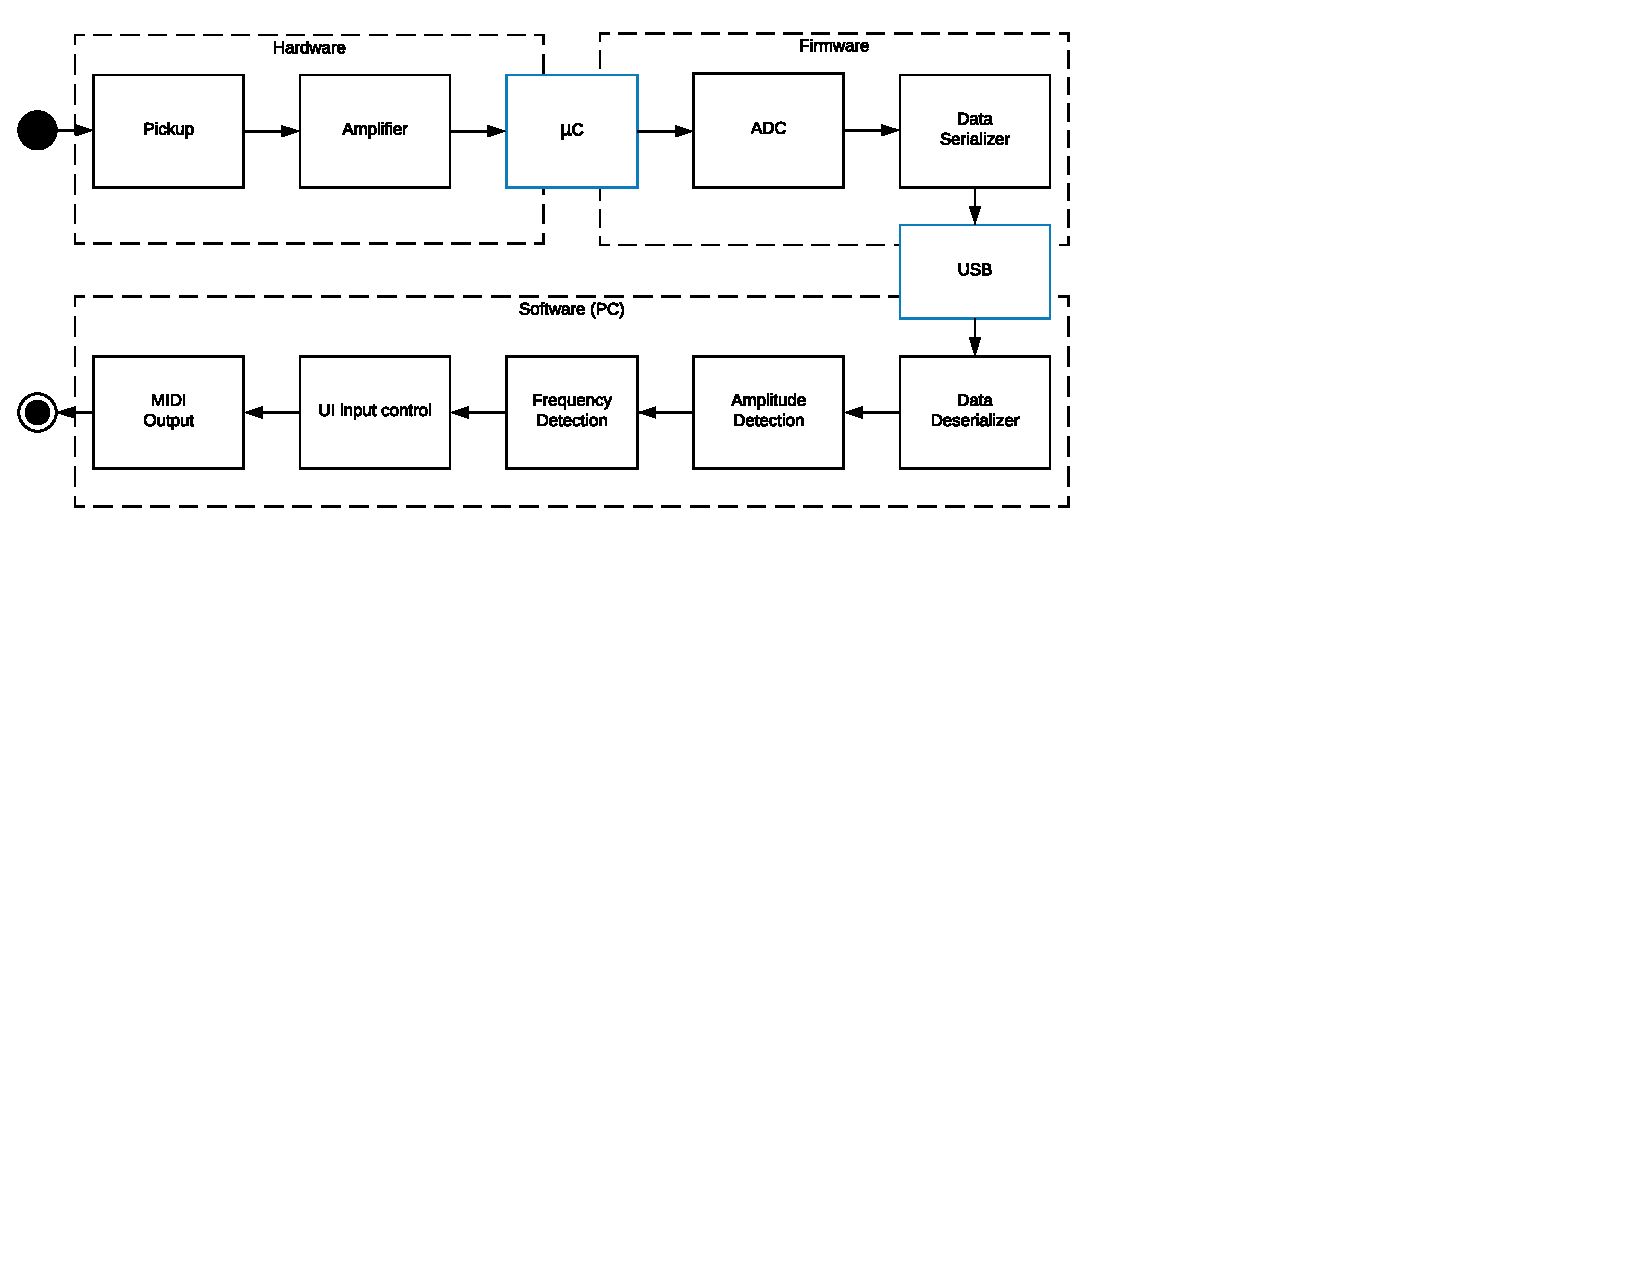
\includegraphics[scale=0.85]{images/system-overview}
  \legend{Source: Authors}
\end{figure}